\documentclass{article}
\usepackage{fancyhdr} % Required for custom headers
\usepackage{lastpage} % Required to determine the last page for the footer
\usepackage{extramarks} % Required for headers and footers
\usepackage{graphicx} % Required to insert images
\usepackage[fleqn]{amsmath}
\usepackage[cs4size,UTF8,winfonts,heading=true]{ctex}
\usepackage{times}
\usepackage{floatrow}
\usepackage{longtable,multirow,booktabs}
\usepackage[compact]{titlesec}         % you need this package

% Margins
\topmargin=-0.45in
\evensidemargin=0in
\oddsidemargin=0in
\textwidth=6.5in
\textheight=9.0in
\headsep=0.25in
\headheight=13pt

\linespread{1.1} % Line spacing

% Set up the header and footer
\pagestyle{fancy}
\lhead{网络安全一班} % Top left header
\chead{\hmwkTitle} % Top center head
\rhead{3019244283 谢远峰 } % Top right header
\renewcommand\headrulewidth{0.4pt} % Size of the header rule
\renewcommand\footrulewidth{0.4pt} % Size of the footer rule
\renewcommand{\normalsize}{\fontsize{12pt}{\baselineskip}\selectfont}

%--Edit Title, Author and Date here
\newcommand{\hmwkTitle}{编译原理-语法分析\\自底向上} % Assignment title
\newcommand{\hmwkClassTime}{\today} % Class/lecture time
\newcommand{\hmwkAuthorName}{网安一班\ 3019244283\ 谢远峰 } % Your name


\title{
\vspace{2in}
\Huge{\textbf{\hmwkTitle}}\\
\vspace{2.5in}
}
\author{\textbf{\hmwkAuthorName}}
\date{\hmwkClassTime}

%------------------------------------------------------------------

\begin{document}
\maketitle
\newpage
\noindent
一.考虑文法$G_{1}为:\quad E \rightarrow E+T|T  \qquad T \rightarrow T*F|F \qquad F \rightarrow (E)|i$\\
(1)证明E+T*F是它的一个句型,指出这个句型的所有短语,直接短语和句柄\\
\begin{center}
    \begin{tabular}{|c|c|}\hline
        E                   & 短语                    \\\hline
        $\Rightarrow E+T$   & $\underline{E+T}$       \\\hline
        $\Rightarrow E+T*F$ & $\underline{T*F},E+T*F$ \\\hline
    \end{tabular}
\end{center}

短语:$T*F,T*F,E+T*F$直接短语:$T*F$\qquad 句柄:$E,T,F$

\noindent
二.考虑文法$G_{2}为:\quad S \rightarrow a|\Lambda |(T)  \qquad T \rightarrow T,S|S $\\
(1)给出 (((a, a),$\Lambda$,(a)),a)的最右推导\\
(2)给出 (((a, a),$\Lambda$,(a)),a)的规范归约约 ,即 “移进 归约”的过程。\\
(3)根据$G_{2}$的算符优先关系表(表1),给出输入串(a,(a, a))的算符优先分析过程。\\
(1)\vspace{-1cm}
\begin{align*}
    \setlength{\abovedisplayskip}{0pt}
    \setlength{\belowdisplayskip}{3pt}
     & S \Rightarrow (T) \Rightarrow (T,S) \Rightarrow (T,a) \Rightarrow ((T),a) \Rightarrow ((T),a) \Rightarrow ((T,S),a) \Rightarrow ((T,(T)),a)        \\
     & \Rightarrow ((T,(a)),a) \Rightarrow ((T,S,(a)),a) \Rightarrow ((T,\Lambda,(a)),a)\Rightarrow ((S,\Lambda,(a)),a) \Rightarrow (((T),\Lambda,(a)),a) \\
     & \Rightarrow (((T,S),\Lambda,(a)),a) \Rightarrow (((T,a),\Lambda,(a)),a) \Rightarrow (((S,a),\Lambda,(a)),a) \Rightarrow (((a,a),\Lambda,(a)),a)
\end{align*}
\vspace{-1cm}
\noindent
(2)
\begin{center}
    \setlength{\abovedisplayskip}{0pt}
    \begin{longtable}{|c|l|r|c|}\hline
        \setlength{\belowdisplayskip}{0pt}
        步骤 & 符号栈          & 输入串                      & 所用产生式                           \\\hline
        0    & $\#$            & $(((a,a),\Lambda,(a)),a)\#$ & 移进                                 \\\hline
        1    & $\#($           & $((a,a),\Lambda,(a)),a)\#$  & 移进                                 \\\hline
        2    & $\#(($          & $(a,a),\Lambda,(a)),a)\#$   & 移进                                 \\\hline
        3    & $\#((($         & $a,a),\Lambda,(a)),a)\#$    & 移进                                 \\\hline
        4    & $\#(((a$        & $,a),\Lambda,(a)),a)\#$     & 归约$a\rightarrow S \rightarrow T$   \\\hline
        5    & $\#(((T,$       & $a),\Lambda,(a)),a)\#$      & 移进                                 \\\hline
        6    & $\#(((T,a$      & $),\Lambda,(a)),a)\#$       & 归约$a\rightarrow S$                 \\\hline
        7    & $\#(((T,S$      & $),\Lambda,(a)),a)\#$       & 归约$T,S\rightarrow T$               \\\hline
        8    & $\#(((T$        & $),\Lambda,(a)),a)\#$       & 移进                                 \\\hline
        9    & $\#(((T)$       & $,\Lambda,(a)),a)\#$        & 归约$(T)\rightarrow S$               \\\hline
        11   & $\#((S$         & $,\Lambda,(a)),a)\#$        & 归约$S\rightarrow T$                 \\\hline
        12   & $\#((T$         & $,\Lambda,(a)),a)\#$        & 移进                                 \\\hline
        13   & $\#((T,$        & $\Lambda,(a)),a)\#$         & 移进                                 \\\hline
        14   & $\#((T,\Lambda$ & $,(a)),a)\#$                & 归约$\Lambda \rightarrow S $         \\\hline
        15   & $\#((T,S$       & $,(a)),a)\#$                & 归约$T,S\rightarrow T$               \\\hline
        16   & $\#((T$         & $,(a)),a)\#$                & 移进                                 \\\hline
        17   & $\#((T,$        & $(a)),a)\#$                 & 移进                                 \\\hline
        18   & $\#((T,($       & $a)),a)\#$                  & 移进                                 \\\hline
        19   & $\#((T,(a$      & $)),a)\#$                   & 归约$a \rightarrow S \rightarrow T$  \\\hline
        20   & $\#((T,(T$      & $)),a)\#$                   & 移进                                 \\\hline
        21   & $\#((T,(T)$     & $),a)\#$                    & 归约$(T) \rightarrow S$              \\\hline
        22   & $\#((T,S$       & $),a)\#$                    & 归约$T,S\rightarrow T$               \\\hline
        23   & $\#((T$         & $),a)\#$                    & 移进                                 \\\hline
        24   & $\#((T)$        & $,a)\#$                     & 归约$(T)\rightarrow S \rightarrow T$ \\\hline
        25   & $\#(T$          & $,a)\#$                     & 移进                                 \\\hline
        26   & $\#(T,$         & $a)\#$                      & 移进                                 \\\hline
        27   & $\#(T,a$        & $)\#$                       & 归约$a \rightarrow S$                \\\hline
        28   & $\#(T,S$        & $)\#$                       & 归约$T,S \rightarrow T$              \\\hline
        29   & $\#(T$          & $)\#$                       & 移进                                 \\\hline
        30   & $\#(T)$         & $\#$                        & 归约$(T) \rightarrow S$              \\\hline
        31   & $\#S$           & $\#$                        & 接受                                 \\\hline
    \end{longtable}
\end{center}
\vspace{-1cm}
(3)\vspace{-1cm}
\begin{center}
    \begin{longtable}{|c|l|c|c|r|c|}\hline
        步骤 & 符号栈      & 优先关系 & 当前符号 & 输入串        & 所用产生式             \\\hline
        0    & $\#$        & <        & (        & $(a,(a,a))\#$ & 移进                   \\\hline
        1    & $\#($       & <        & a        & $a,(a,a))\#$  & 移进                   \\\hline
        2    & $\#(a$      & >        & ,        & $,(a,a))\#$   & 归约$a\rightarrow S$   \\\hline
        3    & $\#(S$      & <        & ,        & $,(a,a))\#$   & 移进                   \\\hline
        4    & $\#(S,$     & <        & (        & $,(a,a))\#$   & 移进                   \\\hline
        5    & $\#(S,$     & <        & (        & $(a,a))\#$    & 移进                   \\\hline
        6    & $\#(S,($    & <        & a        & $a,a))\#$     & 移进                   \\\hline
        7    & $\#(S,(a$   & >        & ,        & $,a))\#$      & 归约$a\rightarrow S$   \\\hline
        8    & $\#(S,(S$   & <        & ,        & $,a))\#$      & 移进                   \\\hline
        9    & $\#(S,(S,$  & <        & a        & $a))\#$       & 移进                   \\\hline
        10   & $\#(S,(S,a$ & >        & )        & $a))\#$       & 归约$a\rightarrow S$   \\\hline
        11   & $\#(T,(T,S$ & >        & )        & $))\#$        & 归约$T,S\rightarrow T$ \\\hline
        12   & $\#(T,(T$   & =        & )        & $))\#$        & 移进                   \\\hline
        13   & $\#(T,(T)$  & >        & )        & $)\#$         & 归约$(T)\rightarrow S$ \\\hline
        14   & $\#(T,S$    & >        & )        & $)\#$         & 归约$T,S\rightarrow T$ \\\hline
        15   & $\#(T$      & =        & )        & $)\#$         & 移进                   \\\hline
        16   & $\#(T)$     & >        & $\#$     & $\#$          & 归约$(T)\rightarrow S$ \\\hline
        17   & $\#S$       & =        & $\#$     & $\#$          & 接受                   \\\hline
    \end{longtable}
\end{center}
\newpage

\noindent
三.考虑文法$G_{3}为:\quad S \rightarrow A  \qquad A \rightarrow Ab|bBa \qquad B \rightarrow aAc|a|aAb $\\
证明$G_{3}$是SLR(1)而不是LR(0)的\\
\begin{minipage}[h]{0.6\linewidth}
    \begin{flushleft}
        $0.S \rightarrow A \qquad 1.A \rightarrow Ab \qquad 2.A  \rightarrow bBa$\\
        $3.B \rightarrow aAc \qquad 4.B \rightarrow a \qquad 5.B  \rightarrow aAb$ \\
        状态5存在“归约-移进”冲突,状态9存在“归约-归约”冲突,因此该文法不是LR(0)文法\\

        状态5:\\
        $FOLLOW(B)=\{a\},FOLLOW(B)\bigcap \{b\}=\Phi$\\

        状态9:\\
        $FOLLOW(B)=\{a\},FOLLOW(A)=\{\#,b,c\}$\\
        $FOLLOW(B)\bigcap FOLLOW(A)=\Phi$\\

        状态5和状态9的冲突均可以用SLR(1)方法解决\\构造表如下:

        \begin{longtable}{|c|c|c|c|c|c|c|}\hline
            % \caption{构造LR(0)项目集规范族}
            \multirow{2}*{状态} & \multicolumn{4}{|c|}{ACTION} & \multicolumn{2}{c|}{GOTO}                         \\\cline{2-7}
                                & a                            & b                         & c     & $\#$  & A & B \\\hline
            0                   &                              & S2                        &       &       & 1 &   \\\hline
            1                   &                              & S3                        &       & ACC   & 1 &   \\\hline
            2                   & S5                           &                           &       &       &   & 4 \\\hline
            3                   & R1                           & R1                        & R1    & R1    &   &   \\\hline
            4                   & S6                           &                           &       &       &   &   \\\hline
            5                   & R4                           & S2/R4                     & R4    & R4    & 7 &   \\\hline
            6                   & R2                           & R2                        & R2    & R2    &   &   \\\hline
            7                   &                              & S9                        & S8    &       &   &   \\\hline
            8                   & R3                           &                           &       &       &   &   \\\hline
            9                   & R5/R1                        & R5/R1                     & R5/R1 & R5/R1 &   &   \\\hline
        \end{longtable}

        该SLR(1)分析表无重定义,因此该文法是SLR(1)\\
        文法,不是LR(0)文法。
        \vspace{0.5cm}
    \end{flushleft}
\end{minipage}
\hfill
\begin{minipage}[h]{0.4\linewidth}
    \begin{flushright}
        \begin{longtable}{|c|c|c|}\hline
            % \caption{构造LR(0)项目集规范族}
            状态             & 项目集                       & 转换函数    \\\hline
            \multirow{3}*{0} & $S\rightarrow \bullet A $    & $GO[0,A]=1$ \\\cline{2-3}
                             & $A\rightarrow \bullet Ab$    & $GO[0,A]=1$ \\\cline{2-3}
                             & $A\rightarrow \bullet bBa$   & $GO[0,b]=2$ \\\hline
            \multirow{2}*{1} & $S\rightarrow  A\bullet $    & accept      \\\cline{2-3}
                             & $A\rightarrow  A\bullet b$   & $GO[1,b]=3$ \\\hline
            \multirow{4}*{2} & $A\rightarrow  b\bullet Ba $ & $GO[2,B]=4$ \\\cline{2-3}
                             & $B\rightarrow  \bullet aAc$  & $GO[2,a]=5$ \\\cline{2-3}
                             & $B\rightarrow  \bullet a $   & $GO[2,a]=5$ \\\cline{2-3}
                             & $B\rightarrow  \bullet aAb$  & $GO[2,a]=5$ \\\hline
            3                & $A \rightarrow Ab \bullet $  & R1          \\\hline
            4                & $A \rightarrow bB \bullet a$ & GO[4,a]=6   \\\hline
            \multirow{5}*{5} & $B\rightarrow  a\bullet  Ac$ & $GO[5,A]=7$ \\\cline{2-3}
                             & $B\rightarrow  a\bullet $    & R4          \\\cline{2-3}
                             & $B\rightarrow  a\bullet Ab$  & $GO[5,A]=7$ \\\cline{2-3}
                             & $A\rightarrow  \bullet Ab$   & $GO[5,A]=7$ \\\cline{2-3}
                             & $A\rightarrow  \bullet bBa$  & $GO[5,b]=2$ \\\hline
            6                & $A \rightarrow bBa \bullet$  & R2          \\\hline
            \multirow{3}*{7} & $B\rightarrow  aA\bullet c$  & $GO[7,c]=8$ \\\cline{2-3}
                             & $B\rightarrow  aA\bullet b$  & $GO[7,b]=9$ \\\cline{2-3}
                             & $A\rightarrow  A\bullet b$   & $GO[7,b]=9$ \\\hline
            8                & $B \rightarrow aAc \bullet$  & R3          \\\hline
            \multirow{2}*{9} & $B\rightarrow  aAb\bullet $  & R5          \\\cline{2-3}
                             & $A\rightarrow  Ab\bullet $   & R1          \\\hline
        \end{longtable}
    \end{flushright}
\end{minipage}

\newpage
\noindent
四.考虑文法$G_{4}为:\quad S \rightarrow AS|b  \qquad A \rightarrow SA|a$\\
(1)列出$G_{4}$的所有LR(0)项目\\
(2)构造$G_{4}$的项目集规范族及识别活前缀的DFA\\
(3)$G_{4}$是SLR文法么?如果是,构造出它的SLR分析表\\
(3)$G_{4}$是LR(1)的么?\\
(1)\vspace{-1cm}
\begin{center}
    \begin{longtable}{l|l|l}\hline
        0.$S'\rightarrow \bullet S$  & 1.$S'\rightarrow S\bullet $  &                              \\\hline
        2.$S\rightarrow \bullet AS$  & 3.$S\rightarrow  A\bullet S$ & 4.$S\rightarrow  AS\bullet$  \\\hline
        5.$S\rightarrow \bullet b$   & 6.$S\rightarrow  b\bullet$   &                              \\\hline
        7.$A\rightarrow  \bullet SA$ & 8.$A\rightarrow  S\bullet A$ & 9.$A\rightarrow  SA\bullet $ \\\hline
        10.$A\rightarrow  \bullet a$ & 11.$A\rightarrow  a\bullet $ &                              \\\hline
    \end{longtable}
\end{center}
\vspace{-1cm}
(2)\vspace{-1cm}
% \begin{longtable}{|c|c|}\hline
%     项目集                                                                                                                                              & 转换函数        \\\hline
%     $\{S'\rightarrow \bullet S,S\rightarrow \bullet AS,S\rightarrow \bullet b,A\rightarrow \bullet SA,A\rightarrow \bullet a\}$                         & $I_0$           \\\hline
%     $\{A\rightarrow a\bullet \} $                                                                                                                       & $GO(I_0,a)=I_1$ \\\hline
%     $\{S\rightarrow b\bullet\} $                                                                                                                        & $GO(I_0,b)=I_2$ \\\hline
%     $\{S'\rightarrow S\bullet ,A\rightarrow S\bullet A,A\rightarrow \bullet SA,A\rightarrow \bullet a,S\rightarrow \bullet AS,S\rightarrow \bullet b\}$ & $GO(I_0,S)=I_3$ \\\hline
%     $\{S\rightarrow A\bullet S,S\rightarrow \bullet AS,S\rightarrow \bullet b,A\rightarrow \bullet SA,A\rightarrow \bullet a\}$                         & $GO(I_0,A)=I_4$ \\\hline
%     $\{A\rightarrow a\bullet\} $                                                                                                                        & $GO(I_3,a)=I_1$ \\\hline
%     $\{S\rightarrow b\bullet\} $                                                                                                                        & $GO(I_3,b)=I_2$ \\\hline
%     $\{A\rightarrow S\bullet A,S\rightarrow \bullet AS,S\rightarrow \bullet b,A\rightarrow \bullet SA,A\rightarrow \bullet a\} $                        & $GO(I_3,S)=I_5$ \\\hline
%     $\{A\rightarrow SA\bullet ,A\rightarrow S\bullet A,S\rightarrow \bullet AS,S\rightarrow \bullet b,A\rightarrow \bullet SA,A\rightarrow \bullet a\}$ & $GO(I_3,A)=I_6$ \\\hline
%     $\{A\rightarrow a\bullet\} $                                                                                                                        & $GO(I_4,a)=I_1$ \\\hline
%     $\{S\rightarrow b\bullet\} $                                                                                                                        & $GO(I_4,b)=I_2$ \\\hline
%     $\{S\rightarrow AS\bullet,A\rightarrow S\bullet A,S\rightarrow \bullet AS,S\rightarrow \bullet b,A\rightarrow \bullet SA,A\rightarrow \bullet a\} $ & $GO(I_4,S)=I_7$ \\\hline
%     $\{S\rightarrow A\bullet S,S\rightarrow \bullet AS,S\rightarrow \bullet b,A\rightarrow \bullet SA,A\rightarrow \bullet a\} $                        & $GO(I_4,A)=I_4$ \\\hline
%     $\{A\rightarrow a\bullet\} $                                                                                                                        & $GO(I_5,a)=I_1$ \\\hline
%     $\{S\rightarrow b\bullet\} $                                                                                                                        & $GO(I_5,b)=I_2$ \\\hline
%     $\{A\rightarrow S\bullet A,S\rightarrow \bullet AS,S\rightarrow \bullet b,A\rightarrow \bullet SA,A\rightarrow \bullet a\} $                        & $GO(I_5,S)=I_5$ \\\hline
%     $\{A\rightarrow SA\bullet ,A\rightarrow S\bullet A,S\rightarrow \bullet AS,S\rightarrow \bullet b,A\rightarrow \bullet SA,A\rightarrow \bullet a\}$ & $GO(I_5,A)=I_6$ \\\hline
%     $\{A\rightarrow a\bullet\} $                                                                                                                        & $GO(I_6,a)=I_1$ \\\hline
%     $\{S\rightarrow b\bullet\} $                                                                                                                        & $GO(I_6,b)=I_2$ \\\hline
%     $\{S\rightarrow AS\bullet,A\rightarrow S\bullet A,S\rightarrow \bullet AS,S\rightarrow \bullet b,A\rightarrow \bullet SA,A\rightarrow \bullet a\} $ & $GO(I_6,S)=I_7$ \\\hline
%     $\{S\rightarrow A\bullet S,S\rightarrow \bullet AS,S\rightarrow \bullet b,A\rightarrow \bullet SA,A\rightarrow \bullet a\} $                        & $GO(I_6,A)=I_4$ \\\hline
%     $\{A\rightarrow a\bullet\} $                                                                                                                        & $GO(I_7,a)=I_1$ \\\hline
%     $\{S\rightarrow b\bullet\} $                                                                                                                        & $GO(I_7,b)=I_2$ \\\hline
%     $\{A\rightarrow S\bullet A,S\rightarrow \bullet AS,S\rightarrow \bullet b,A\rightarrow \bullet SA,A\rightarrow \bullet a\} $                        & $GO(I_7,S)=I_5$ \\\hline
%     $\{A\rightarrow SA\bullet ,A\rightarrow S\bullet A,S\rightarrow \bullet AS,S\rightarrow \bullet b,A\rightarrow \bullet SA,A\rightarrow \bullet a\}$ & $GO(I_7,A)=I_6$ \\\hline
% \end{longtable}
\begin{center}
    \begin{longtable}{|c|c|c|c|}\hline
        \multicolumn{4}{|c|}{项目集转换}                                      \\\hline
        $GO(I_0,a)=I_1$ & $GO(I_0,b)=I_2$ & $GO(I_0,S)=I_3$ & $GO(I_0,A)=I_4$ \\\hline
        $GO(I_3,a)=I_1$ & $GO(I_3,b)=I_2$ & $GO(I_3,S)=I_5$ & $GO(I_3,A)=I_6$ \\\hline
        $GO(I_4,a)=I_1$ & $GO(I_4,b)=I_2$ & $GO(I_4,S)=I_7$ & $GO(I_4,A)=I_4$ \\\hline
        $GO(I_5,a)=I_1$ & $GO(I_5,b)=I_2$ & $GO(I_5,S)=I_5$ & $GO(I_5,A)=I_6$ \\\hline
        $GO(I_6,a)=I_1$ & $GO(I_6,b)=I_2$ & $GO(I_6,S)=I_7$ & $GO(I_6,A)=I_4$ \\\hline
        $GO(I_7,a)=I_1$ & $GO(I_7,b)=I_2$ & $GO(I_7,S)=I_5$ & $GO(I_7,A)=I_6$ \\\hline
    \end{longtable}
\end{center}
\vspace{-1cm}
其识别活前缀的DFA如下:\\
% \vspace{-1.5cm}
\begin{figure}[ht]
    \centering
    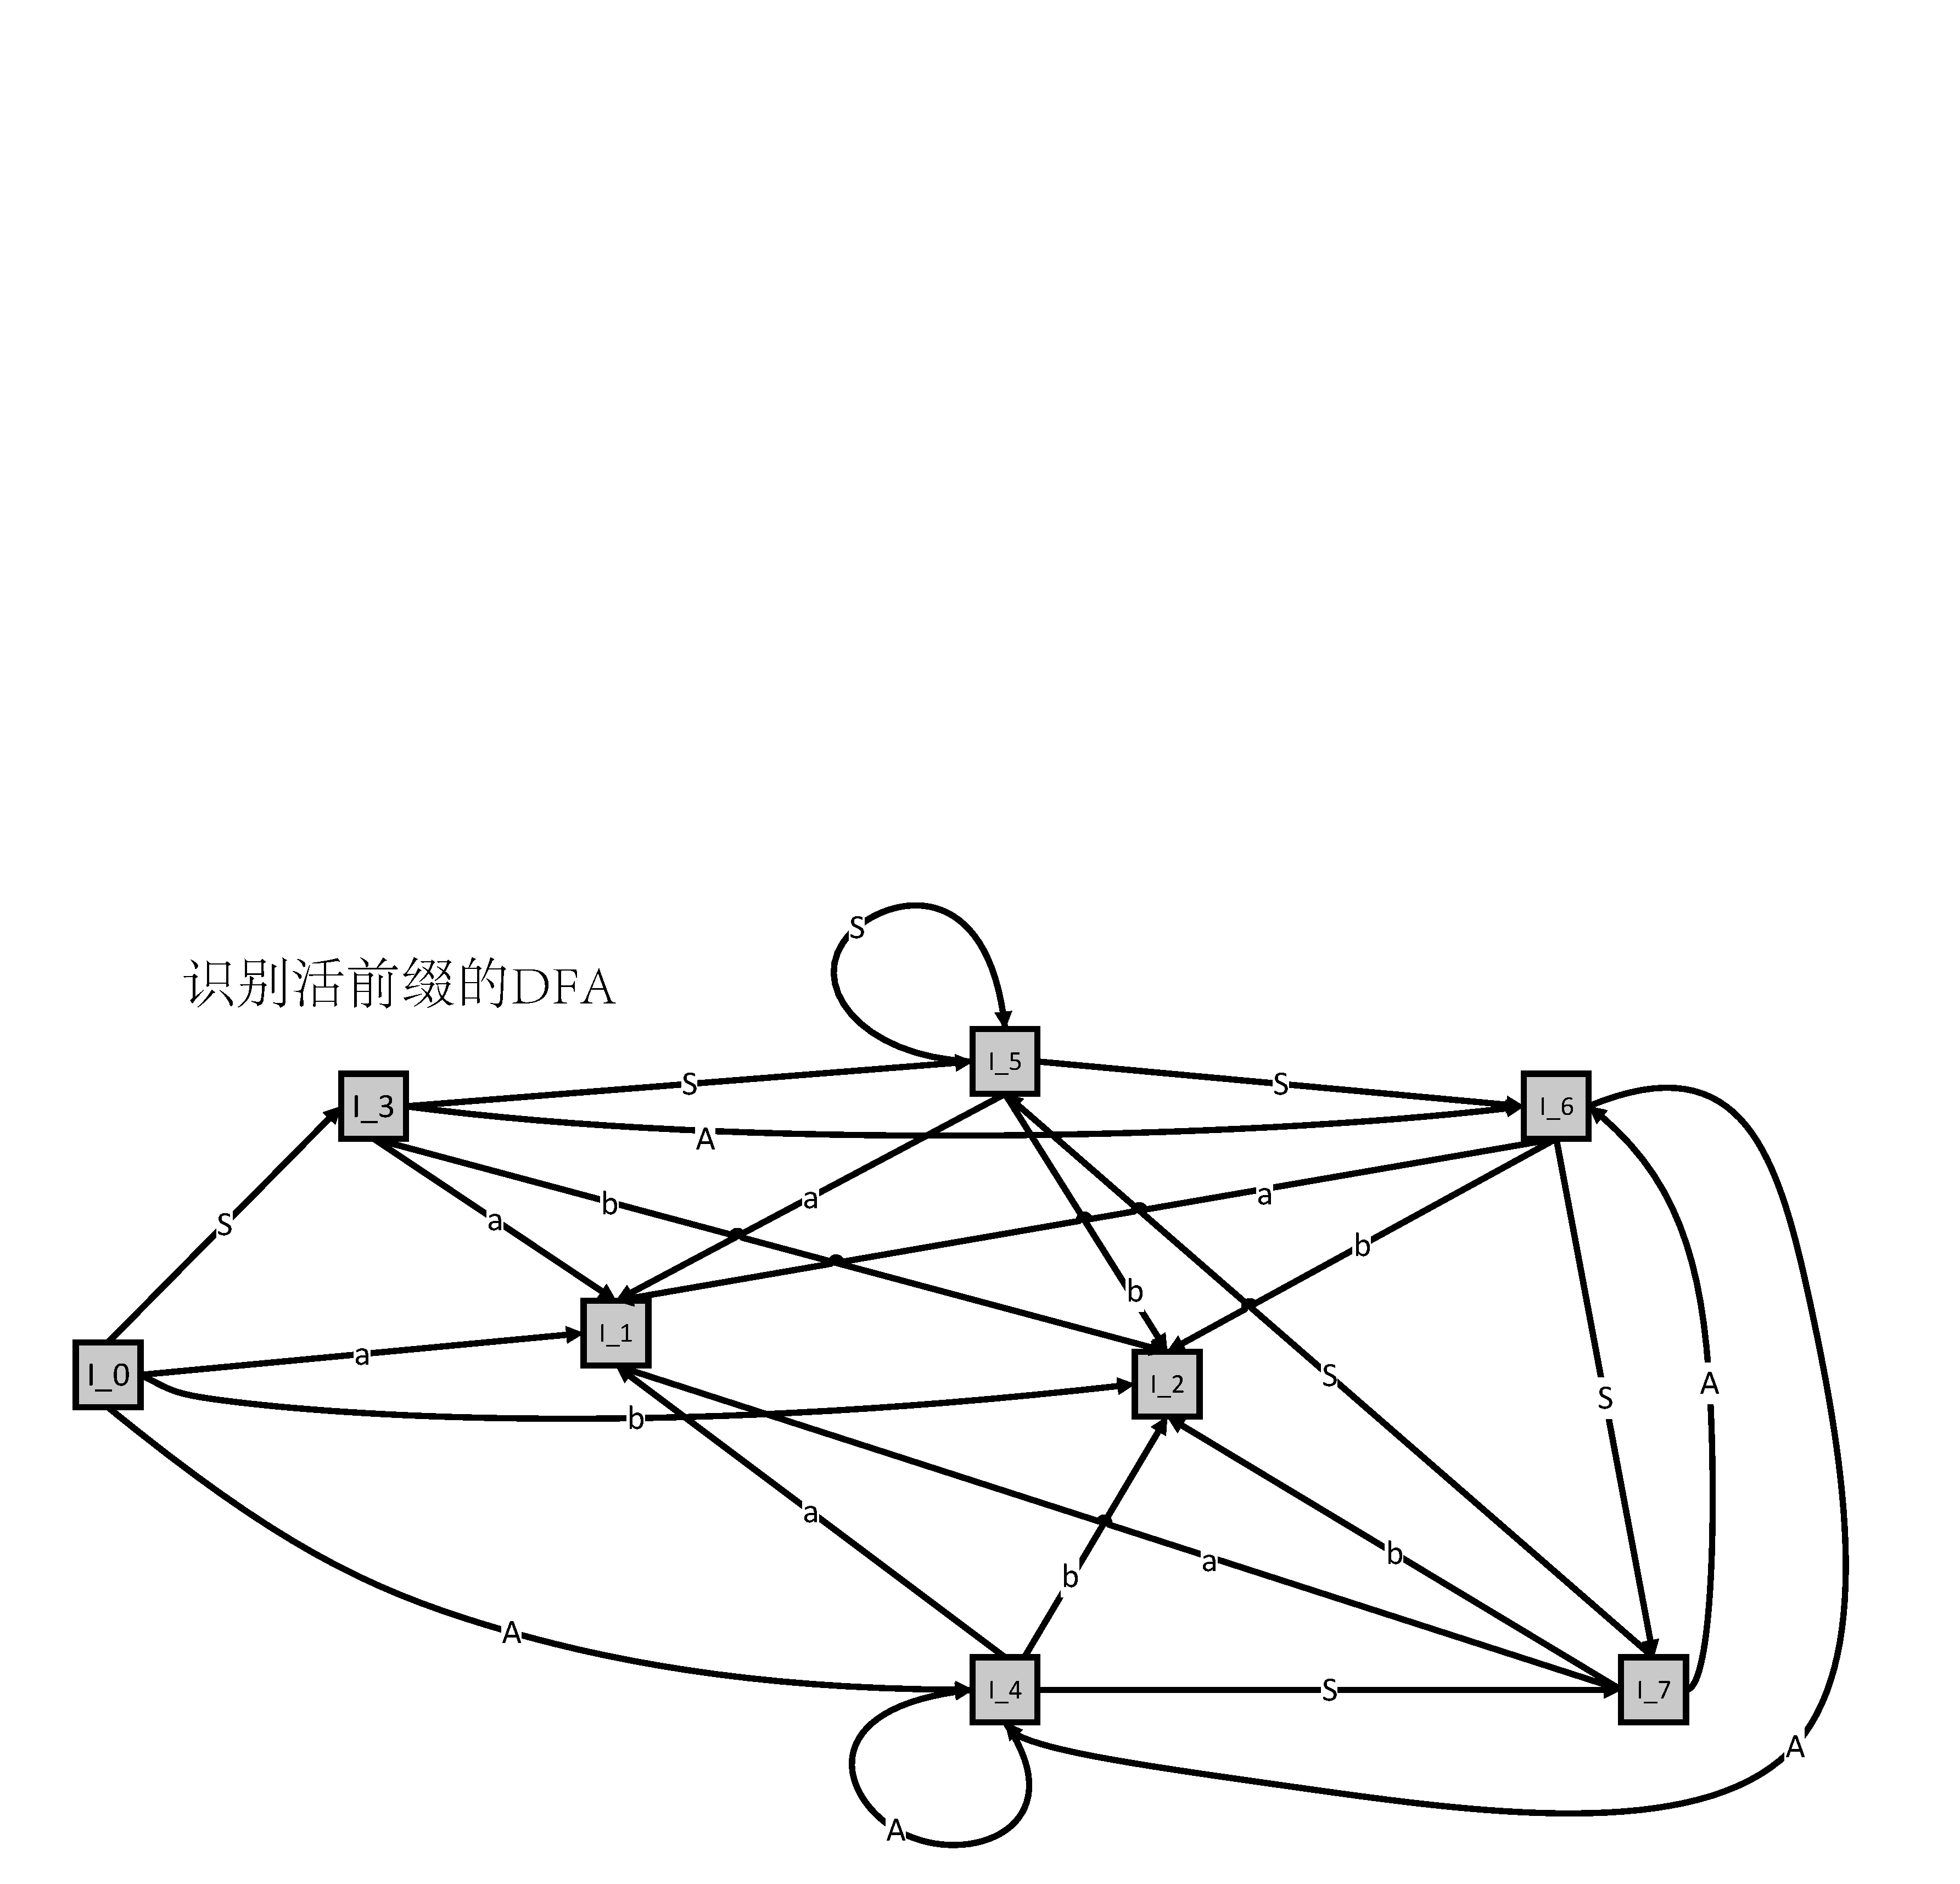
\includegraphics[width=15cm,height=7cm]{DFA.pdf}
    \caption{DFA图}
\end{figure}
\newpage
所以项目集规范族为$C=\{I_0,I_1,I_2,I_3,I_4,I_5,I_6,I_7\}$
\begin{center}
    \begin{longtable}{c|c}\hline
        项目集 & 项目集构成                                                                                                                                          \\\hline
        $I_0$  & $\{S'\rightarrow \bullet S,S\rightarrow \bullet AS,S\rightarrow \bullet b,A\rightarrow \bullet SA,A\rightarrow \bullet a\}$                         \\\hline
        $I_1$  & $\{A\rightarrow a\bullet \} $                                                                                                                       \\\hline
        $I_2$  & $\{S\rightarrow b\bullet\} $                                                                                                                        \\\hline
        $I_3$  & $\{S'\rightarrow S\bullet ,A\rightarrow S\bullet A,A\rightarrow \bullet SA,A\rightarrow \bullet a,S\rightarrow \bullet AS,S\rightarrow \bullet b\}$ \\\hline
        $I_4$  & $\{S\rightarrow A\bullet S,S\rightarrow \bullet AS,S\rightarrow \bullet b,A\rightarrow \bullet SA,A\rightarrow \bullet a\} $                        \\\hline
        $I_5$  & $\{A\rightarrow S\bullet A,S\rightarrow \bullet AS,S\rightarrow \bullet b,A\rightarrow \bullet SA,A\rightarrow \bullet a\} $                        \\\hline
        $I_6$  & $\{A\rightarrow SA\bullet ,S\rightarrow \bullet AS,S\rightarrow A\bullet S,S\rightarrow \bullet b,A\rightarrow \bullet SA,A\rightarrow \bullet a\}$ \\\hline
        $I_7$  & $\{S\rightarrow AS\bullet,A\rightarrow S\bullet A,S\rightarrow \bullet AS,S\rightarrow \bullet b,A\rightarrow \bullet SA,A\rightarrow \bullet a\} $ \\\hline
    \end{longtable}
\end{center}
\vspace{-1cm}


\noindent
(3)不是SLR文法

状态3:6,7有移进归约冲突

状态3:$FOLLOW(S')=\{\#\}$不包含a,b

状态6:$FOLLOW(S)=\{\#,a,b\}$包含a,b,移进归约冲突无法解决

状态7:$FOLLOW(A)=\{a,b\}$,移进归约冲突解决

\noindent
(4)不是LR(1)文法
% \vspace{-1cm}
\begin{longtable}{|c|c|c|c|}\hline

    状态             & 项目集                     & 转换函数      & FOLLOW集合 \\\hline
    \multirow{5}*{0} & $S'\rightarrow \bullet S $ & $GO[0,S]=1$   & $\#$       \\\cline{2-4}
                     & $S\rightarrow \bullet AS$  & $GO[0,A]=1$   & $\#/a/b$   \\\cline{2-4}
                     & $S\rightarrow \bullet b$   & $GO[0,b]=2$   & $\#/a/b$   \\\cline{2-4}
                     & $A\rightarrow \bullet SA$  & $GO[0,S]=1$   & $a/b$      \\\cline{2-4}
                     & $S\rightarrow \bullet a$   & $GO[0,a]=1$   & $a/b$      \\\hline
    1                & $A\rightarrow a\bullet $   & $GO[1,a]=R11$ & $a/b$      \\\hline
    2                & $S\rightarrow b\bullet $   & $GO[2,b]=ACC$ & $\#/a/b$   \\\hline
    \multirow{6}*{3} & $S'\rightarrow S\bullet  $ & $GO[3,S]=R1$  & $\#$       \\\cline{2-4}
                     & $A\rightarrow S\bullet A$  & $GO[3,A]=6$   & $a/b$      \\\cline{2-4}
                     & $A\rightarrow \bullet SA$  & $GO[3,S]=5$   & $a/b$      \\\cline{2-4}
                     & $A\rightarrow \bullet a$   & $GO[3,a]=1$   & $a/b$      \\\cline{2-4}
                     & $S\rightarrow \bullet AS$  & $GO[3,A]=6$   & $a/b$      \\\cline{2-4}
                     & $S\rightarrow \bullet b$   & $GO[3,b]=2$   & $a/b$      \\\hline
    \multirow{5}*{4} & $S\rightarrow A\bullet S $ & $GO[4,A]=4$   & $a/b$      \\\cline{2-4}
                     & $S\rightarrow \bullet AS$  & $GO[4,A]=4$   & $a/b$      \\\cline{2-4}
                     & $S\rightarrow \bullet b$   & $GO[4,b]=2$   & $a/b$      \\\cline{2-4}
                     & $A\rightarrow \bullet SA$  & $GO[4,S]=7$   & $a/b$      \\\cline{2-4}
                     & $A\rightarrow \bullet a$   & $GO[4,a]=1$   & $a/b$      \\\hline
    \multirow{5}*{5} & $A\rightarrow S\bullet A $ & $GO[5,A]=6$   & $a/b$      \\\cline{2-4}
                     & $S\rightarrow \bullet AS$  & $GO[5,A]=6$   & $a/b$      \\\cline{2-4}
                     & $S\rightarrow \bullet b$   & $GO[5,b]=2$   & $a/b$      \\\cline{2-4}
                     & $A\rightarrow \bullet SA$  & $GO[5,S]=5$   & $a/b$      \\\cline{2-4}
                     & $A\rightarrow \bullet a$   & $GO[5,a]=1$   & $a/b$      \\\hline
    \multirow{6}*{6} & $A\rightarrow SA\bullet  $ & $R9$          & $a/b$      \\\cline{2-4}
                     & $A\rightarrow S\bullet A$  & $GO[6,A]=6$   & $a/b$      \\\cline{2-4}
                     & $S\rightarrow \bullet AS$  & $GO[6,A]=6$   & $a/b$      \\\cline{2-4}
                     & $S\rightarrow \bullet b$   & $GO[6,b]=2$   & $a/b$      \\\cline{2-4}
                     & $A\rightarrow \bullet SA$  & $GO[6,S]=7$   & $a/b$      \\\cline{2-4}
                     & $A\rightarrow \bullet a$   & $GO[6,a]=1$   & $a/b$      \\\hline
    \multirow{6}*{7} & $S\rightarrow AS\bullet  $ & $R4$          & $a/b$      \\\cline{2-4}
                     & $A\rightarrow S\bullet A$  & $GO[7,A]=6$   & $a/b$      \\\cline{2-4}
                     & $S\rightarrow \bullet AS$  & $GO[7,A]=6$   & $a/b$      \\\cline{2-4}
                     & $S\rightarrow \bullet b$   & $GO[7,b]=2$   & $a/b$      \\\cline{2-4}
                     & $A\rightarrow \bullet SA$  & $GO[7,S]=5$   & $a/b$      \\\cline{2-4}
                     & $A\rightarrow \bullet a$   & $GO[7,a]=1$   & $a/b$      \\\hline
\end{longtable}
对于状态6,因为包含项目$[A\rightarrow SA\bullet\qquad a/b]$,所以遇到符号a或b时,应该用$A\rightarrow SA$进行归约。又因为状态6包含项目$[A\rightarrow \bullet a \qquad a/b]$,所以遇到搜索符号a时,应当移进。存在“移进-归约”矛盾,所以这个文法不是LR(1)文法。
\end{document}